\documentclass{TDP003mall}
\usepackage[utf8]{inputenc}
\usepackage[swedish]{babel}
\usepackage{graphicx}


\newcommand{\version}{Version 1.1}
\author{Daniel Huber, \url{danhu849@liu.se}\\
  Jens Öhnell, \url{jenoh242@liu.se}}
\title{LOFI-prototyp}
\date{2020-09-17}
\rhead{Daniel Huber\\
Jens Öhnell}



\begin{document}
\projectpage
\section{Revisionshistorik}
\begin{table}[!h]
\begin{tabularx}{\linewidth}{|l|X|l|}
\hline
Ver. & Revisionsbeskrivning & Datum \\\hline
1.1 & Rättade till bildernas orientering & 200917 \\\hline
1.0 & LOFI-prototyp & 200917 \\\hline
\end{tabularx}
\end{table}

\section{Inledning}
Första bilden föreställer det tema och upplägg vi valt att ha på ''riktigt''. På grund av sjukdom kunde tyvärr inte samtliga sidor sammanställas i tid och har därför ritats för hand. Läsaren ombedes ha den första bilden i åtanke gällande färgkomplexitet och utformning för resterande skisser.

Förs musen över de senaste projektbilderna på hemsidan kommer det upp lite info om dem i utrymmet bilderna tar. Alla saker som hänvisas som länkar är klickbara. Oavsett sida kan besökaren alltid klicka på hemsidans titel för att komma till /. Knapparna för social media öppnar nya tabbar till respektive.

Sökfältet högst upp till höger har ingen ''sök-knapp'' utan det förväntas av användaren att trycka ENTER för att komma vidare. Söksidan har liksom tekniksidan också en scroll-bar. Projekten i sökresultaten går att klicka på för att komma till projektets sida. I övre högra delen av söksidan går det att sortera på bokstavsordning, projekt-id och datum de lades in i systemet.

Varje projektsidas bilder går att klicka på för att få dem i större format. I botten på projektsidan finns tags som består av tekniker. Dessa är klickbara och leder till tekniksidan.

På tekniksidan finns färgkodade knappar som färgläggs vid klick. Vid klick återfås en lista lik sökresultaten, men där projektbeskrivningen är utbytt mot en visuell representation av vilka tekniker som använts och i hur stort omfång. Markeras flera knappar samtidigt uppdateras sökresultaten, men inte hela sidan. Sökresultaten sorteras med de markerade teknikerna högst upp.

Vid fel eller inkorrekta inmatningar omdirigeras användaren till en 404 sida där de presenteras med en klickbar tillbakaknapp och information om vad som gick fel.

\newpage

\section{Visuell Presentation}
\begin{figure}[h]
  \centerline{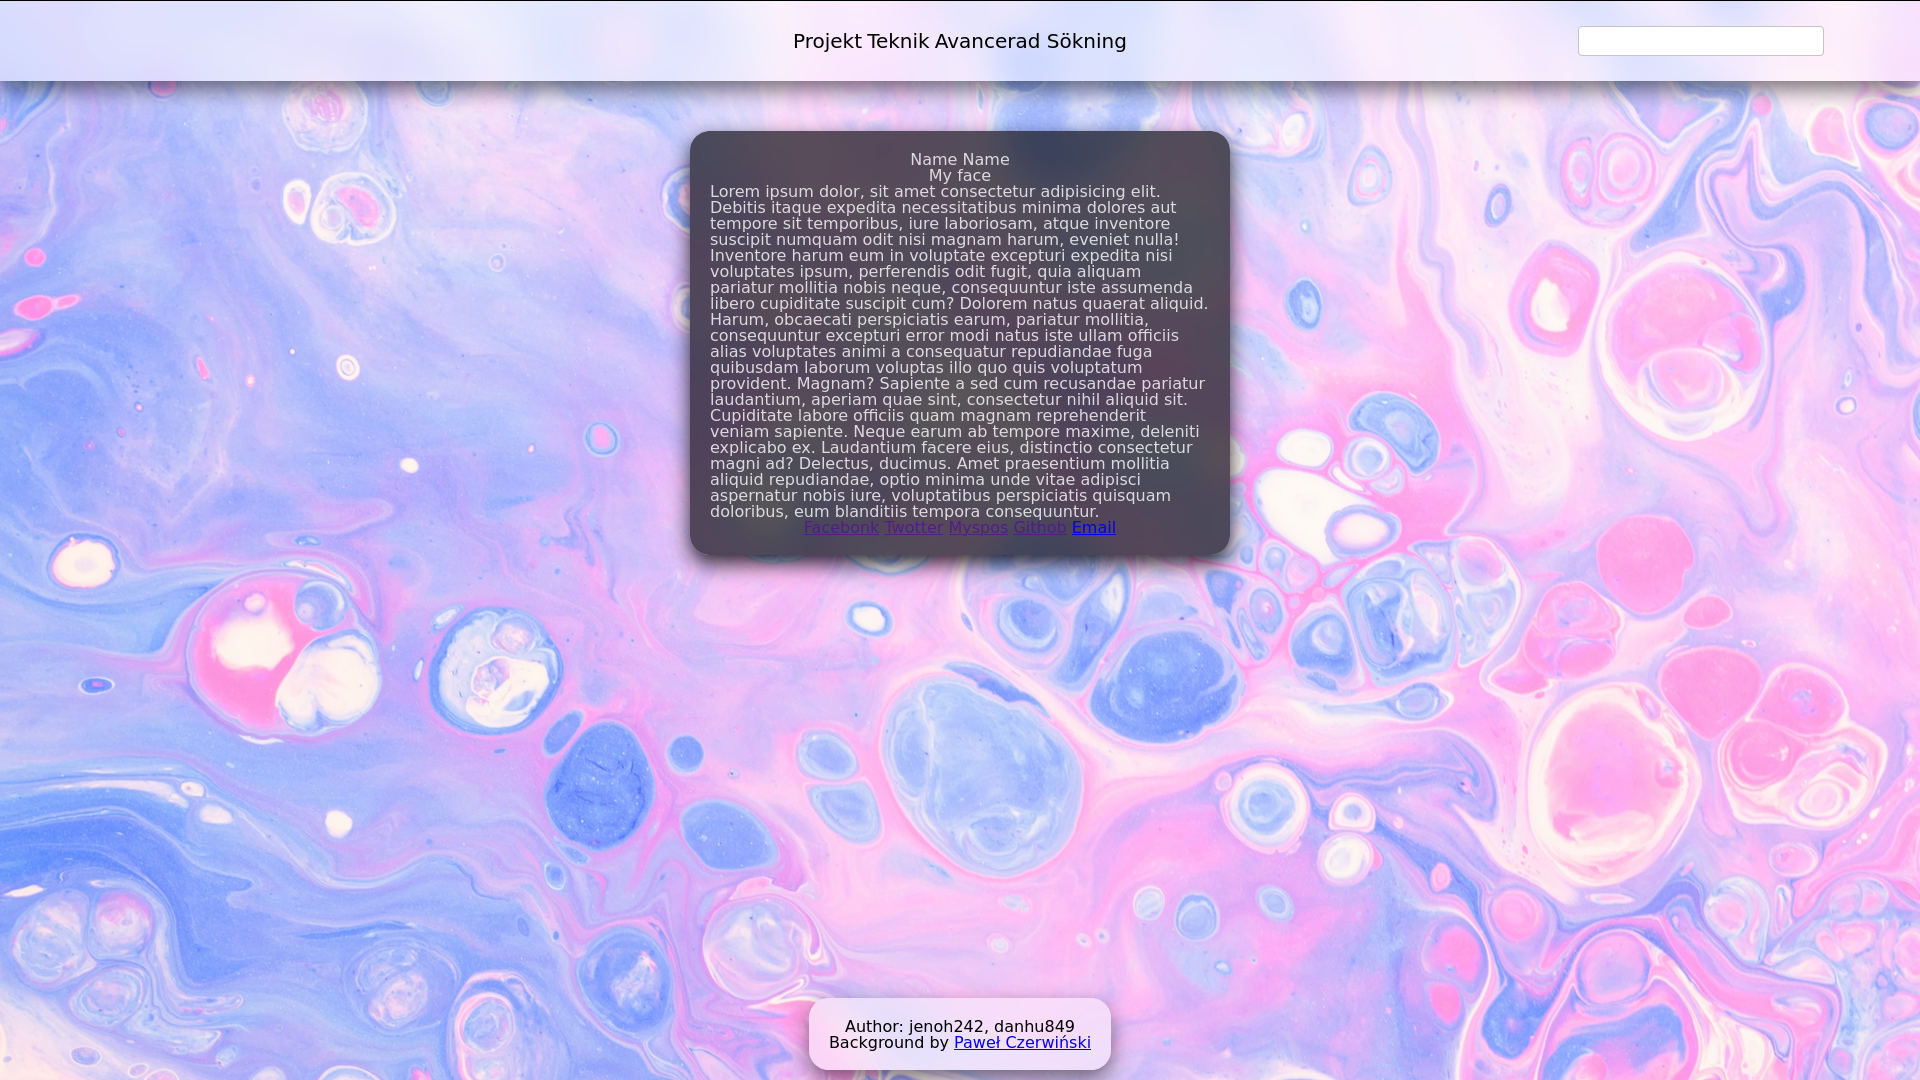
\includegraphics[width=\textwidth]{/home/danhu849/Downloads/Homepage_theme.png}}
  \caption{Färgkod och tema.}
  \label{fig}
\end{figure}

\begin{figure}[h]
  \centerline{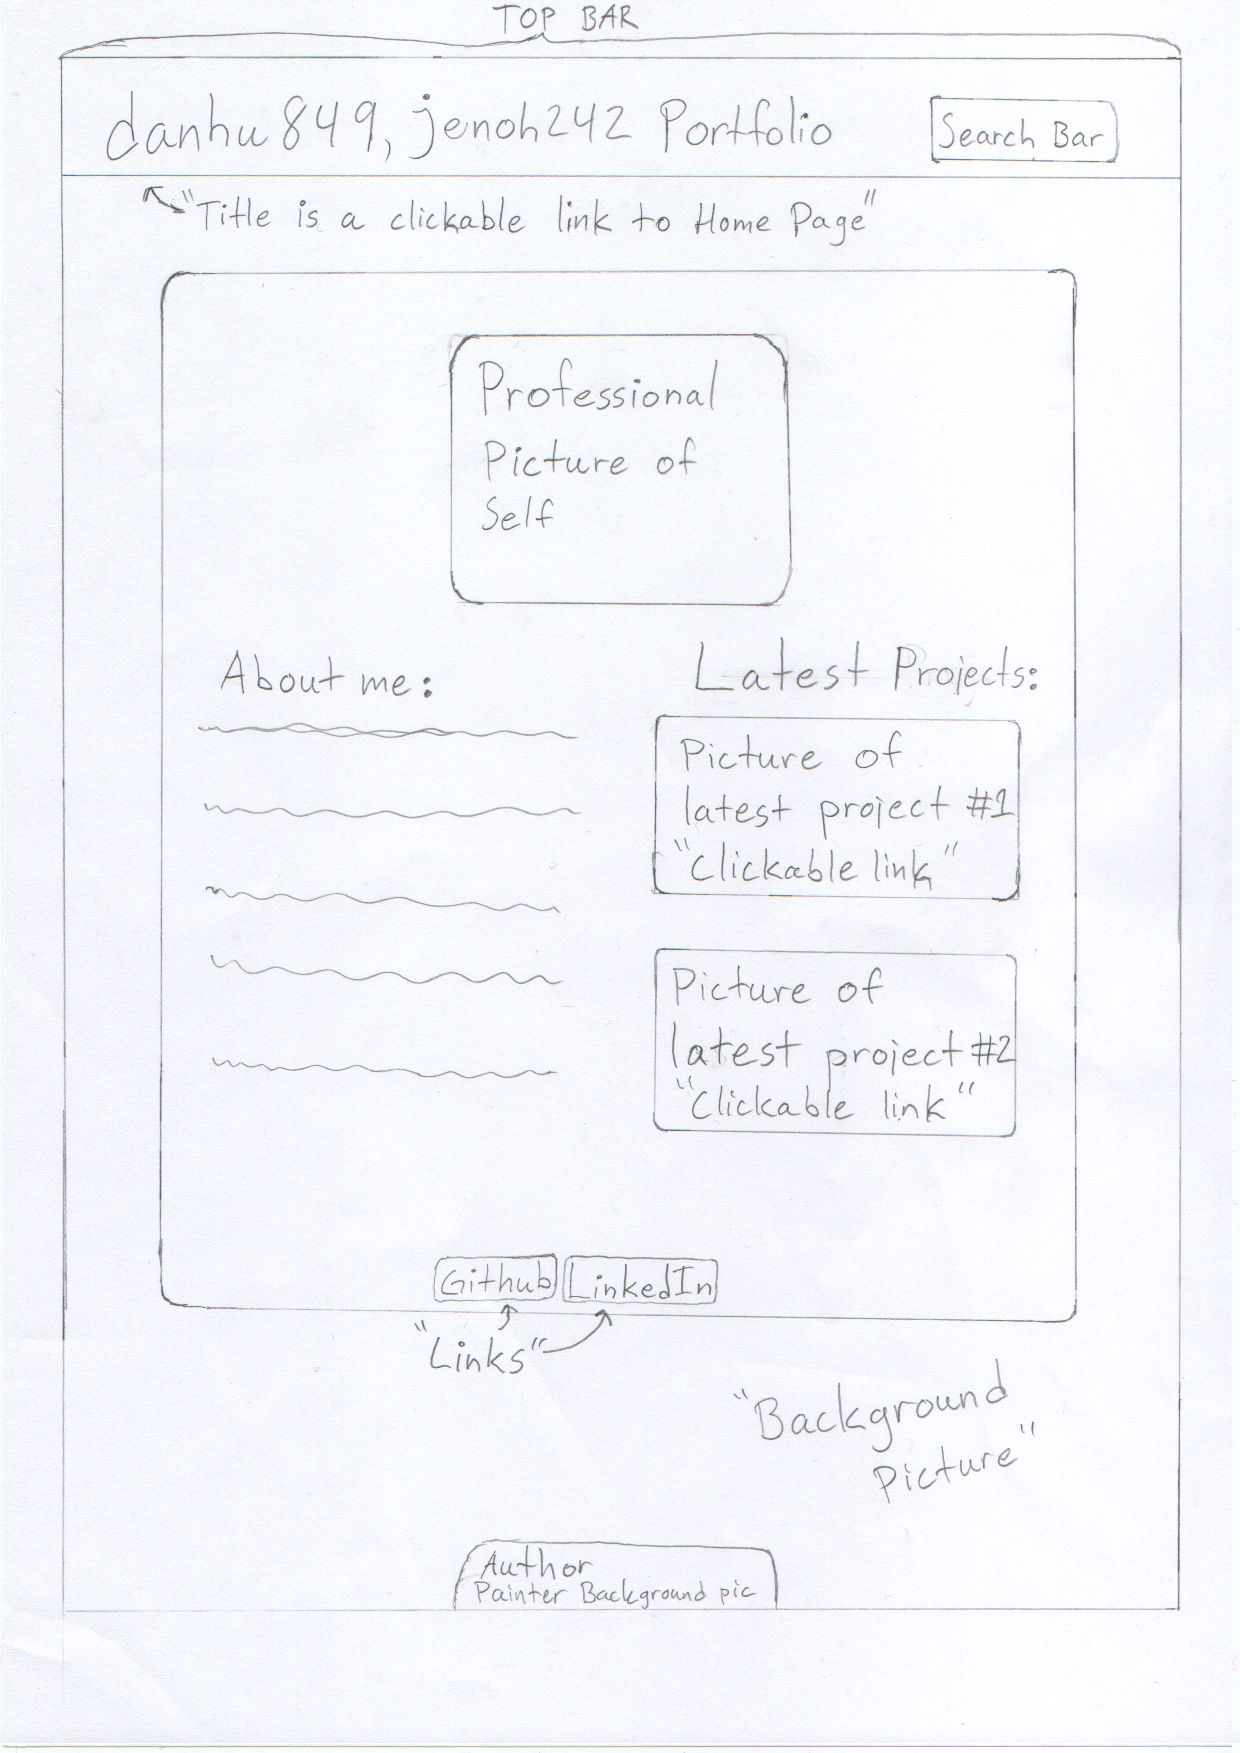
\includegraphics[width=\textwidth, height=20cm]{/home/danhu849/Downloads/home.jpg}}
  \caption{Hemsidan /}
  \label{fig}
\end{figure}

\begin{figure}[h]
  \centerline{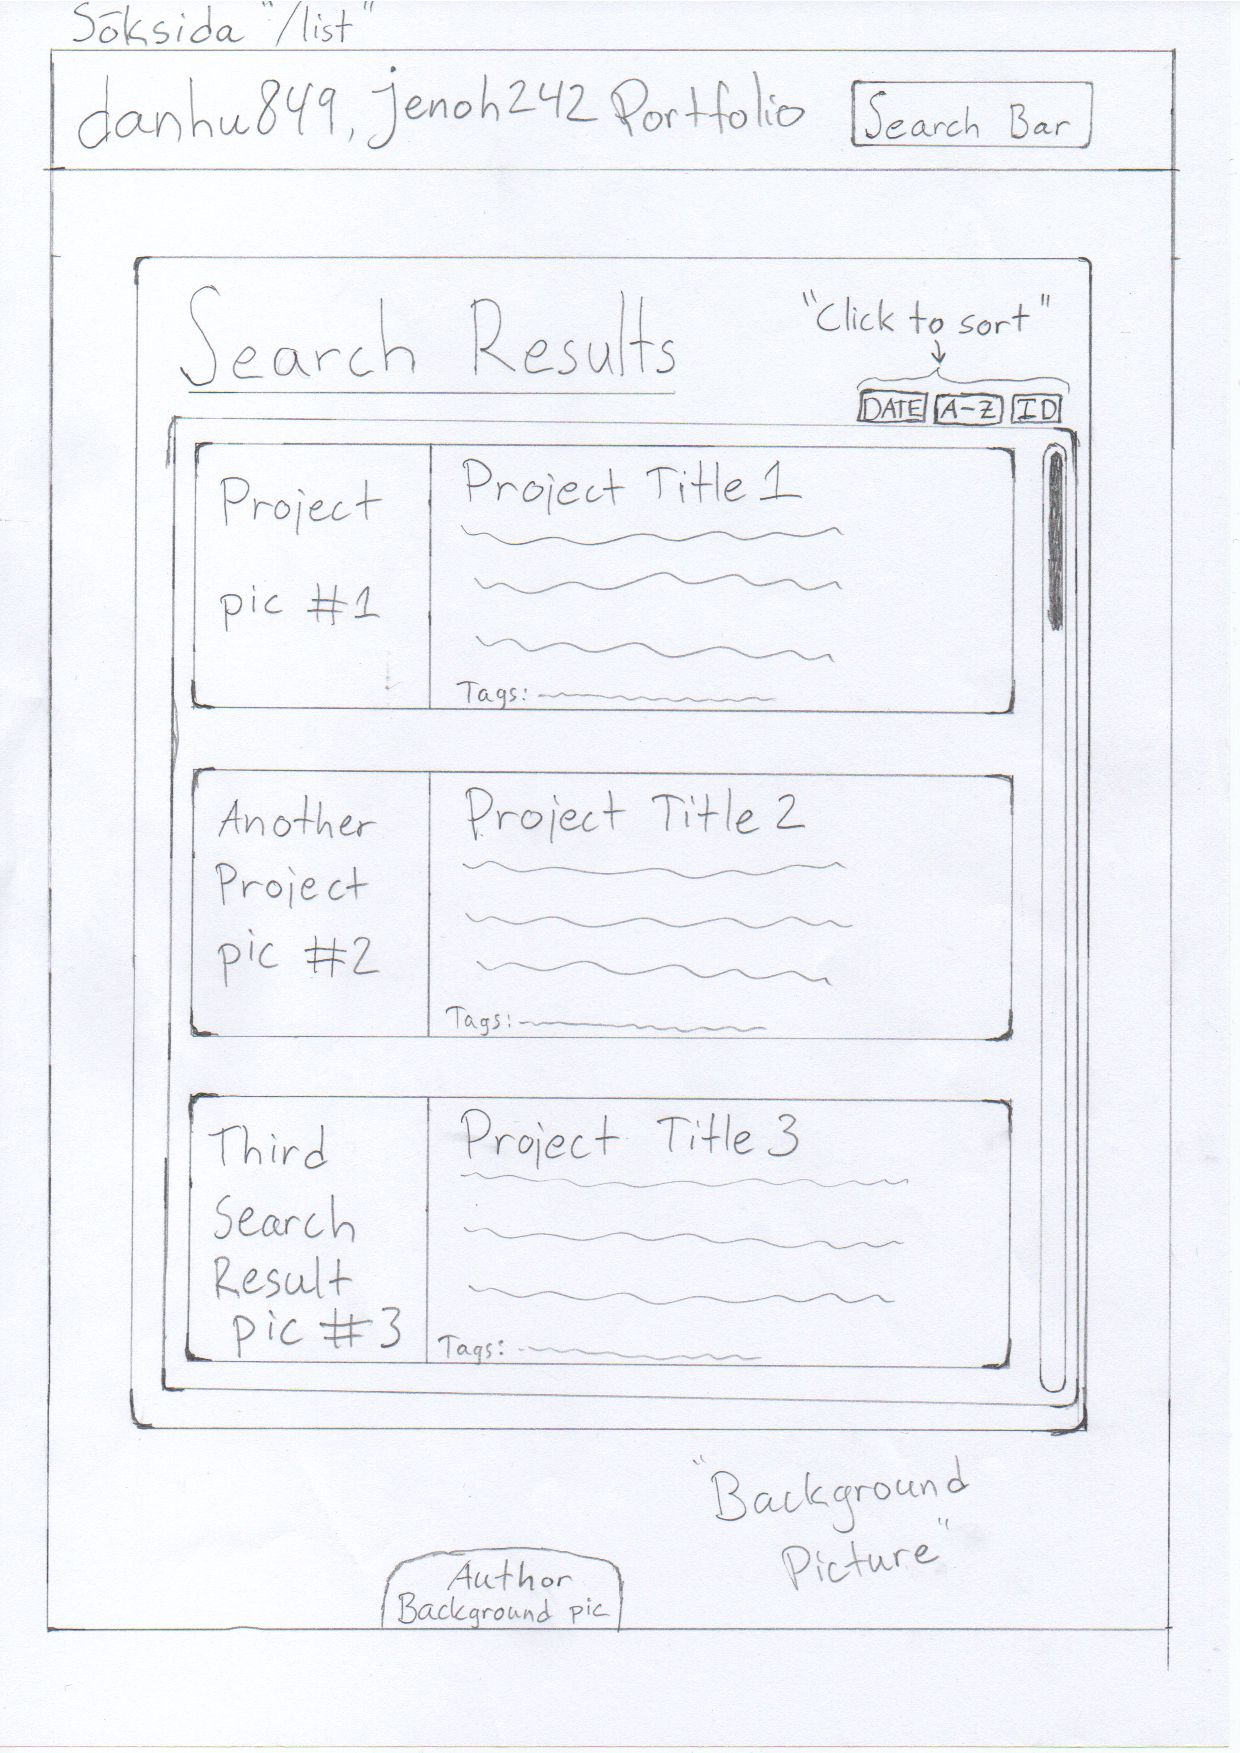
\includegraphics[width=\textwidth, height=20cm]{/home/danhu849/Downloads/search.jpg}}
  \caption{Söksidan /list}
  \label{fig}
\end{figure}

\begin{figure}[h]
  \centerline{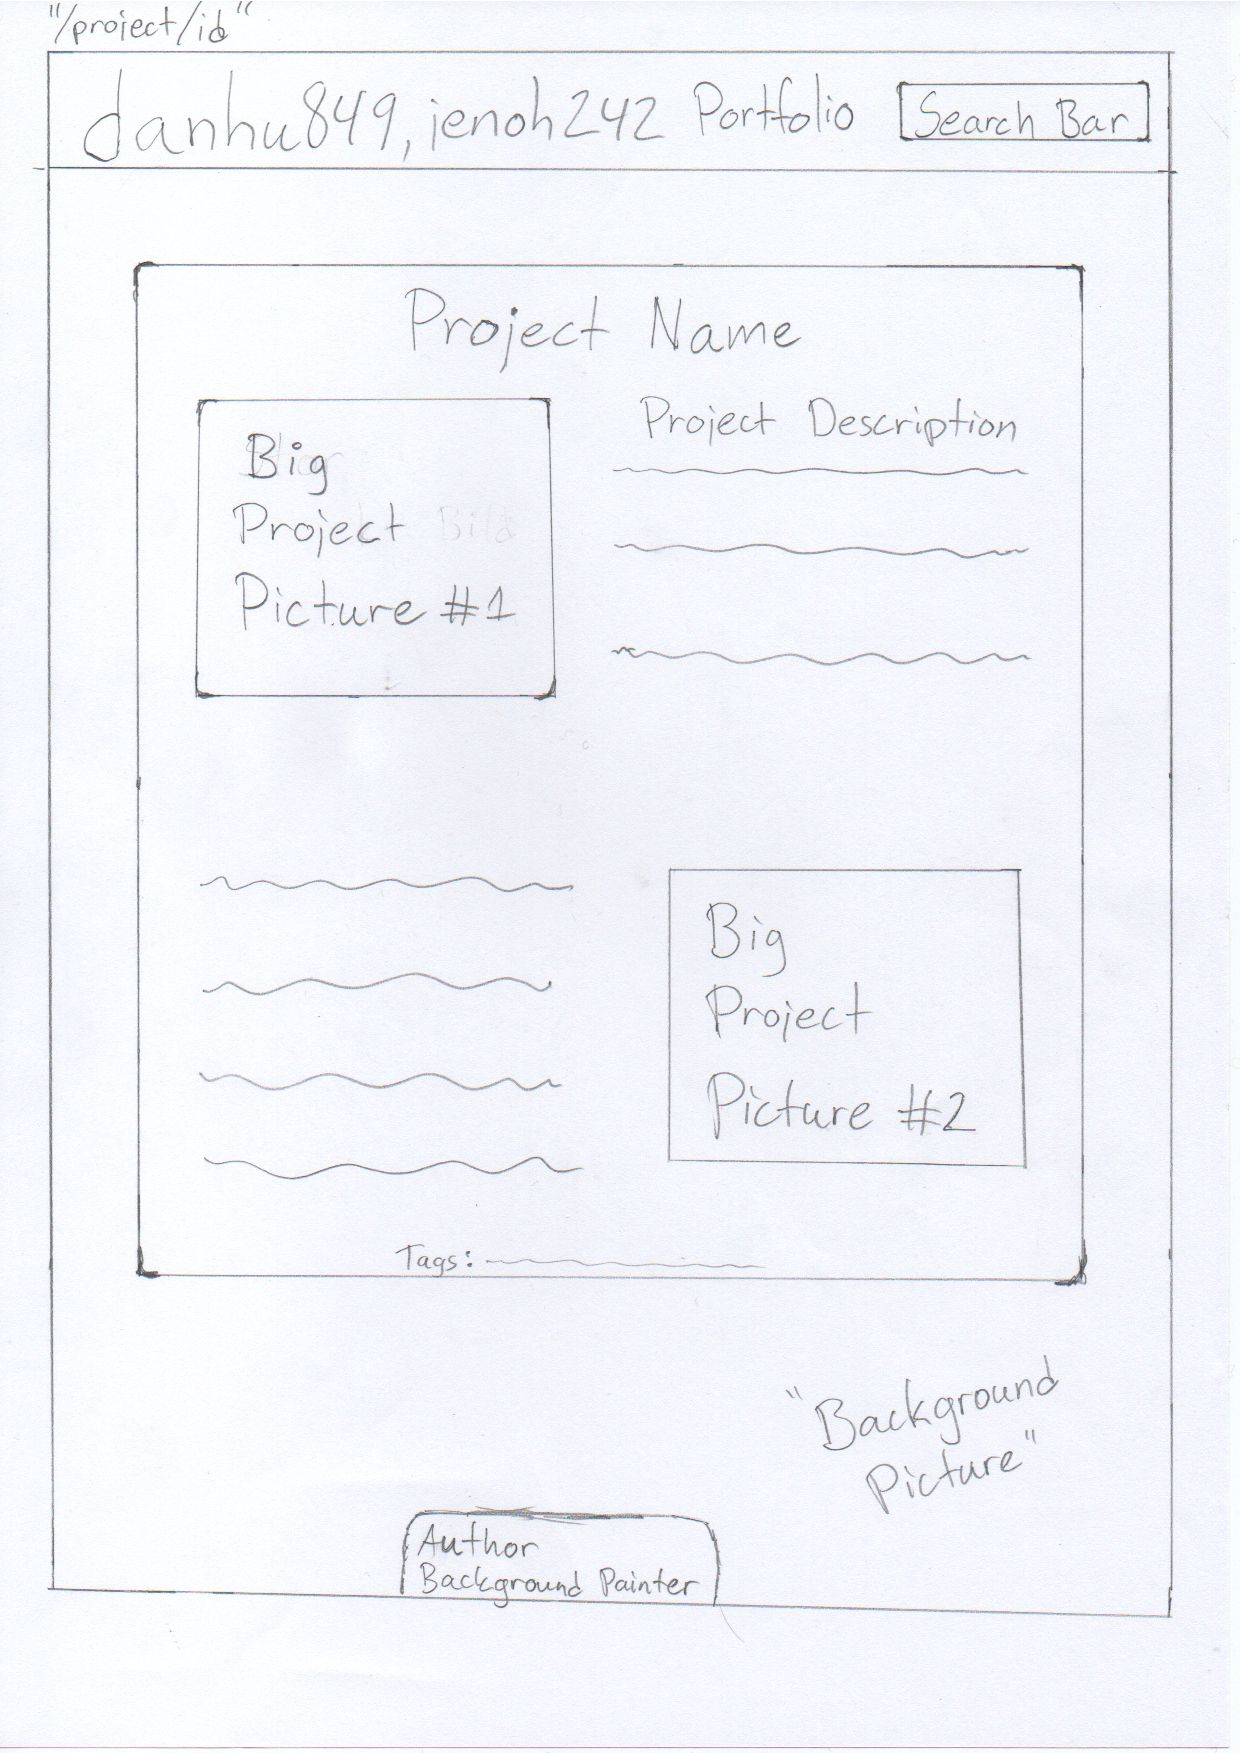
\includegraphics[width=\textwidth, height=20cm]{/home/danhu849/Downloads/project.jpg}}
  \caption{Projektsidan /projekt/id}
  \label{fig}
\end{figure}

\begin{figure}[h]
  \centerline{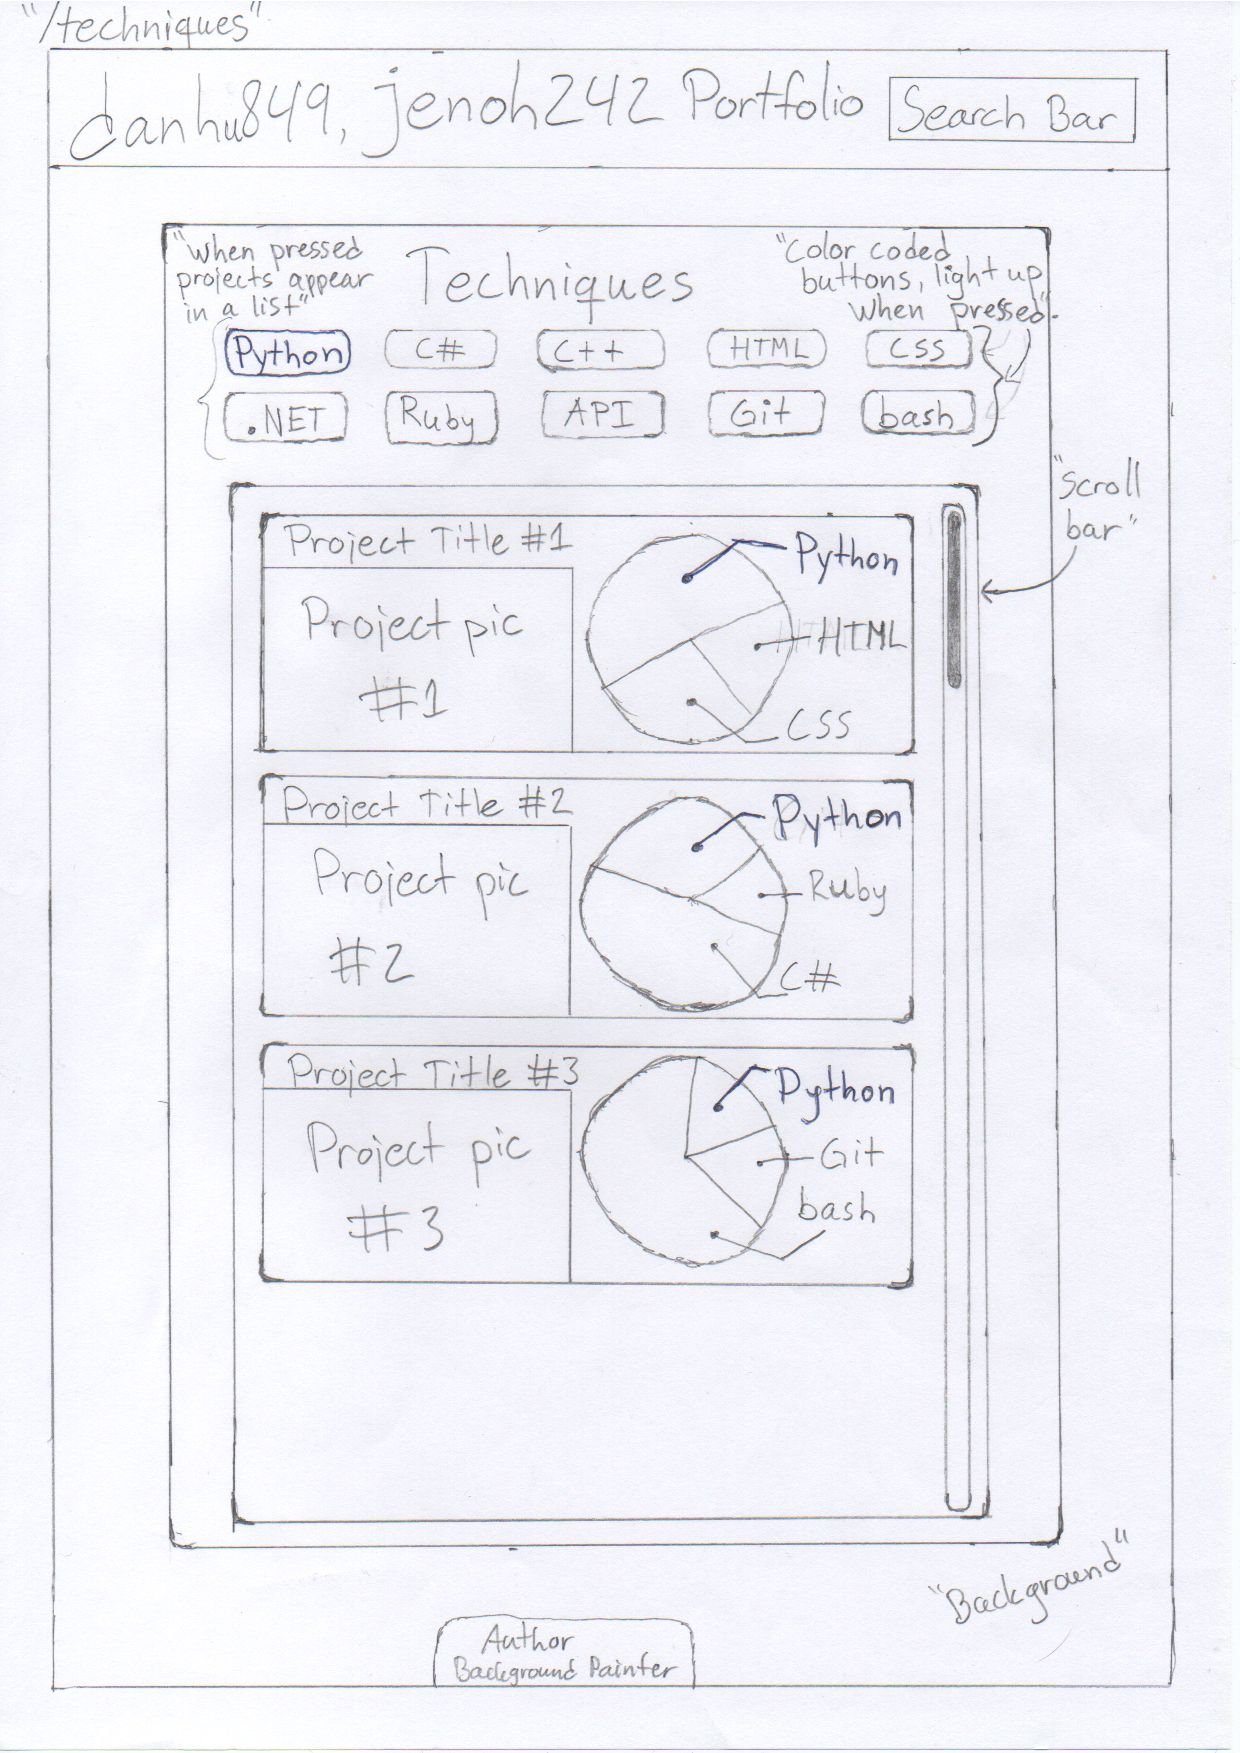
\includegraphics[width=\textwidth, height=20cm]{/home/danhu849/Downloads/techniques.jpg}}
  \caption{Tekniksidan /techniques}
  \label{fig}
\end{figure}

\begin{figure}[h]
  \centerline{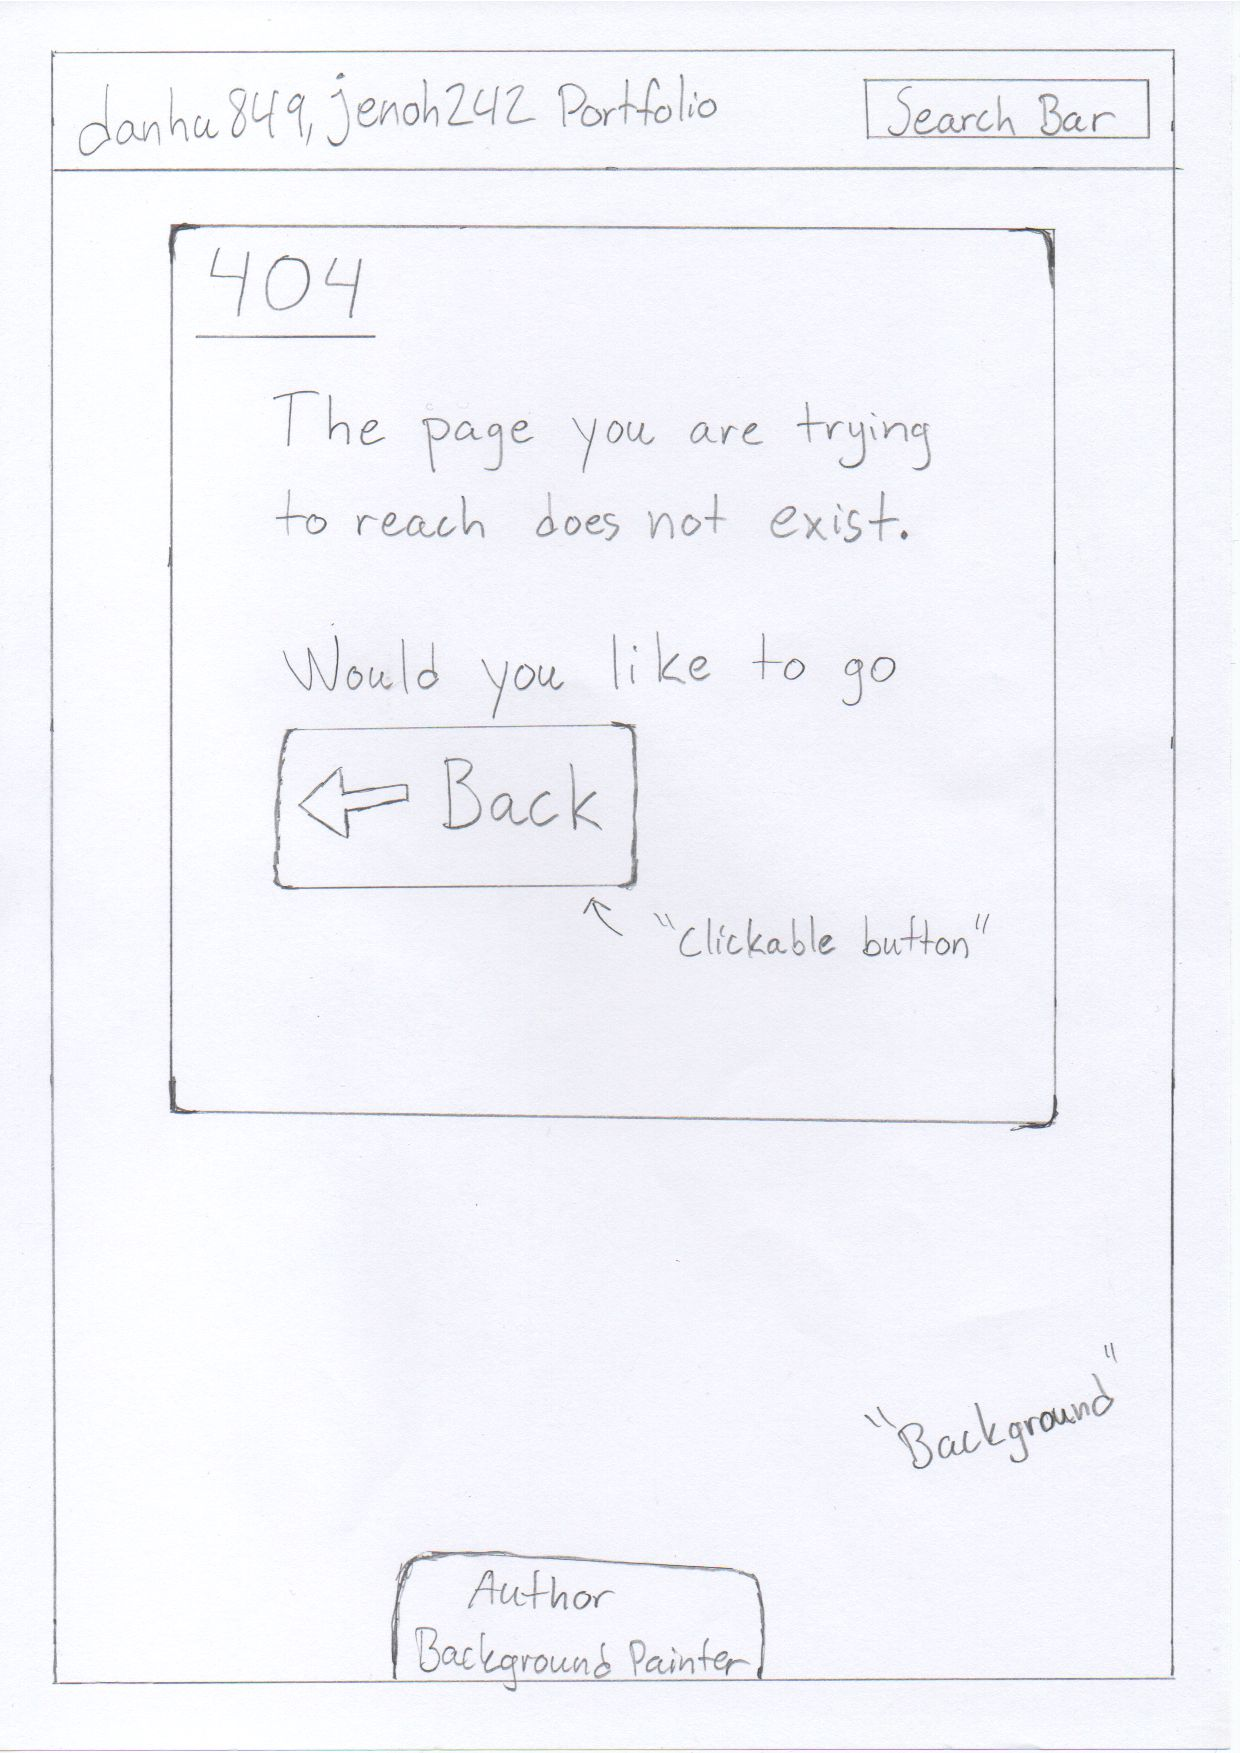
\includegraphics[width=\textwidth, height=20cm]{/home/danhu849/Downloads/404.jpg}}
  \caption{404-sidan}
  \label{fig}
\end{figure}



\end{document}
